\section{Experimental methods}
\label{sec:alkbw:exp}

\subsection{Materials}

In all tests, LR6 alkaline AA batteries were used. The structure of each cell is comprised of (from the center of the cell out) a brass current collecting pin, a Zn/KOH/PVA gel anode, a cellulose separator, a MnO2/graphite cathode, and a stainless steel can. The structure is detailed clearly in Fig.~\ref{fig:aaschem}.

To compare EAToF and EDXRD results, the LR6 alkaline cells used were Duracell MN1500 AA batteries with a nominal voltage of 1.5 V and nominal capacity of 2850 mAh.

To compare brands, a set of LR6 alkaline cells comprised of Duracell QU1500 AA (Quantum), Duracell MN1500 AA (Coppertop), CVS 1500 AA (CVS), and Fujitsu G+ (Fujitsu) AA batteries were tested. All cells had a nominal voltage of 1.5 V and a nominal capacity of 2850 mAh. Cells were weighed using a Metler-Toledo lab balance accurate to 0.1 mg.

\subsection{Ultrasonic interrogation}

Commercially available alkaline Zn-\ce{MnO2} AA batteries were used in this study. Duracell MN1500 AA batteries were discharged using a using a Neware BT3000-8 cycler at rates of 143, 200, 300 and 400 mA, in order to match rates used for in situ EDXRD studies, while all battery brands were discharged at 143 and 400 mA for the battery brand comparison. Cells were subjected to a 10 minute rest at open circuit voltage before discharge, and a 30 minute rest after discharge. During discharge, batteries were ultrasonically interrogated using an Olympus EPOCH 600 ultrasonic flaw detector with two 0.25 in. 2.25 MHz transducers. Tests were performed in transmission mode, using one transducer as the pulser and the other as the receiver. Glycerin was used as an acoustic couplant to minimize the sound speed mismatch between the transducer and the battery. Transducers were held in place using screw pressure inside a custom-designed cell holder printed using a Formlabs Form1+ 3D printer. An experimental schematic is shown in Fig.~\ref{fig:alkbwschem}. For the brand comparison test, a multiplexing circuit was used to automate measurements so all cells could be run concurrently. Custom-written Python software was used to control the EPOCH 600 using Pithy, a cloud-based Python solution.~\cite{Steingart_undated-rr} The incident pulse was 445 ns in length, and the resulting transmission waveform was measured out to 20 μs. Measurements were performed every 30 seconds. The resulting waveforms were then analyzed using Python scripts to track waveform evolution as well as total transmitted signal amplitude. A period from 4 $\upmu$s to 20 $\upmu$s was plotted as the required amplification due to the introduction of the multiplexing circuit amplified the low ToF incident to the point of signal saturation. Data analysis in the absence of the multiplexing circuit have showed the region from 0 $\upmu$s to 4 $\upmu$s to not contain pertinent data, so we feel comfortable with our decision to truncate the dataset. 

\begin{figure}[htb]
  \centering
    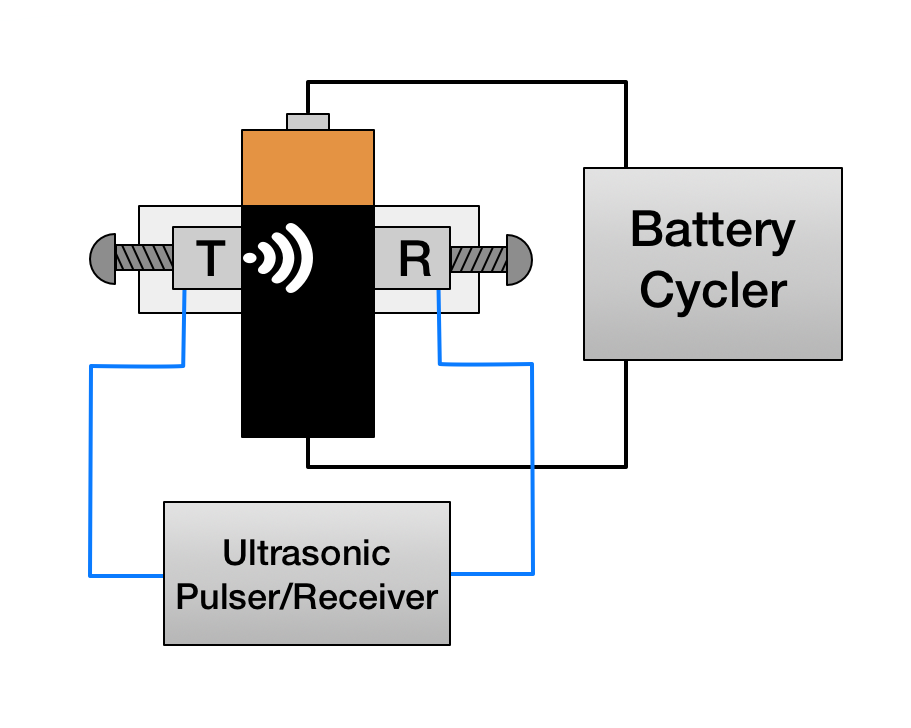
\includegraphics[width=0.80\textwidth]{ch5-alkbw/images/ExpSchem.png}
    \caption[Schematic of experimental setup for ultrasonic interrogation of alkaline AA batteries.]{Schematic of experimental setup for ultrasonic interrogation of alkaline AA batteries, with relevant parts labeled. T and R refer to the transmitting and receiving ultrasonic transducers, respectively.}
    \label{fig:alkbwschem}
\end{figure}

\subsection{Energy dispersive x-ray diffraction}

EDXRD was performed at Beamline X17B1 of the National Synchrotron Light Source (NSLS) at Brookhaven National Lab. Beamline X17B1 is an energy-dispersive x-ray line capable of measuring internal structural changes in a discrete volume. Duracell alkaline AA batteries were analyzed using methodology that has been described in detail by Gallaway et al.~\cite{gallaway}